\begin{figure}[hbtp]
\centering
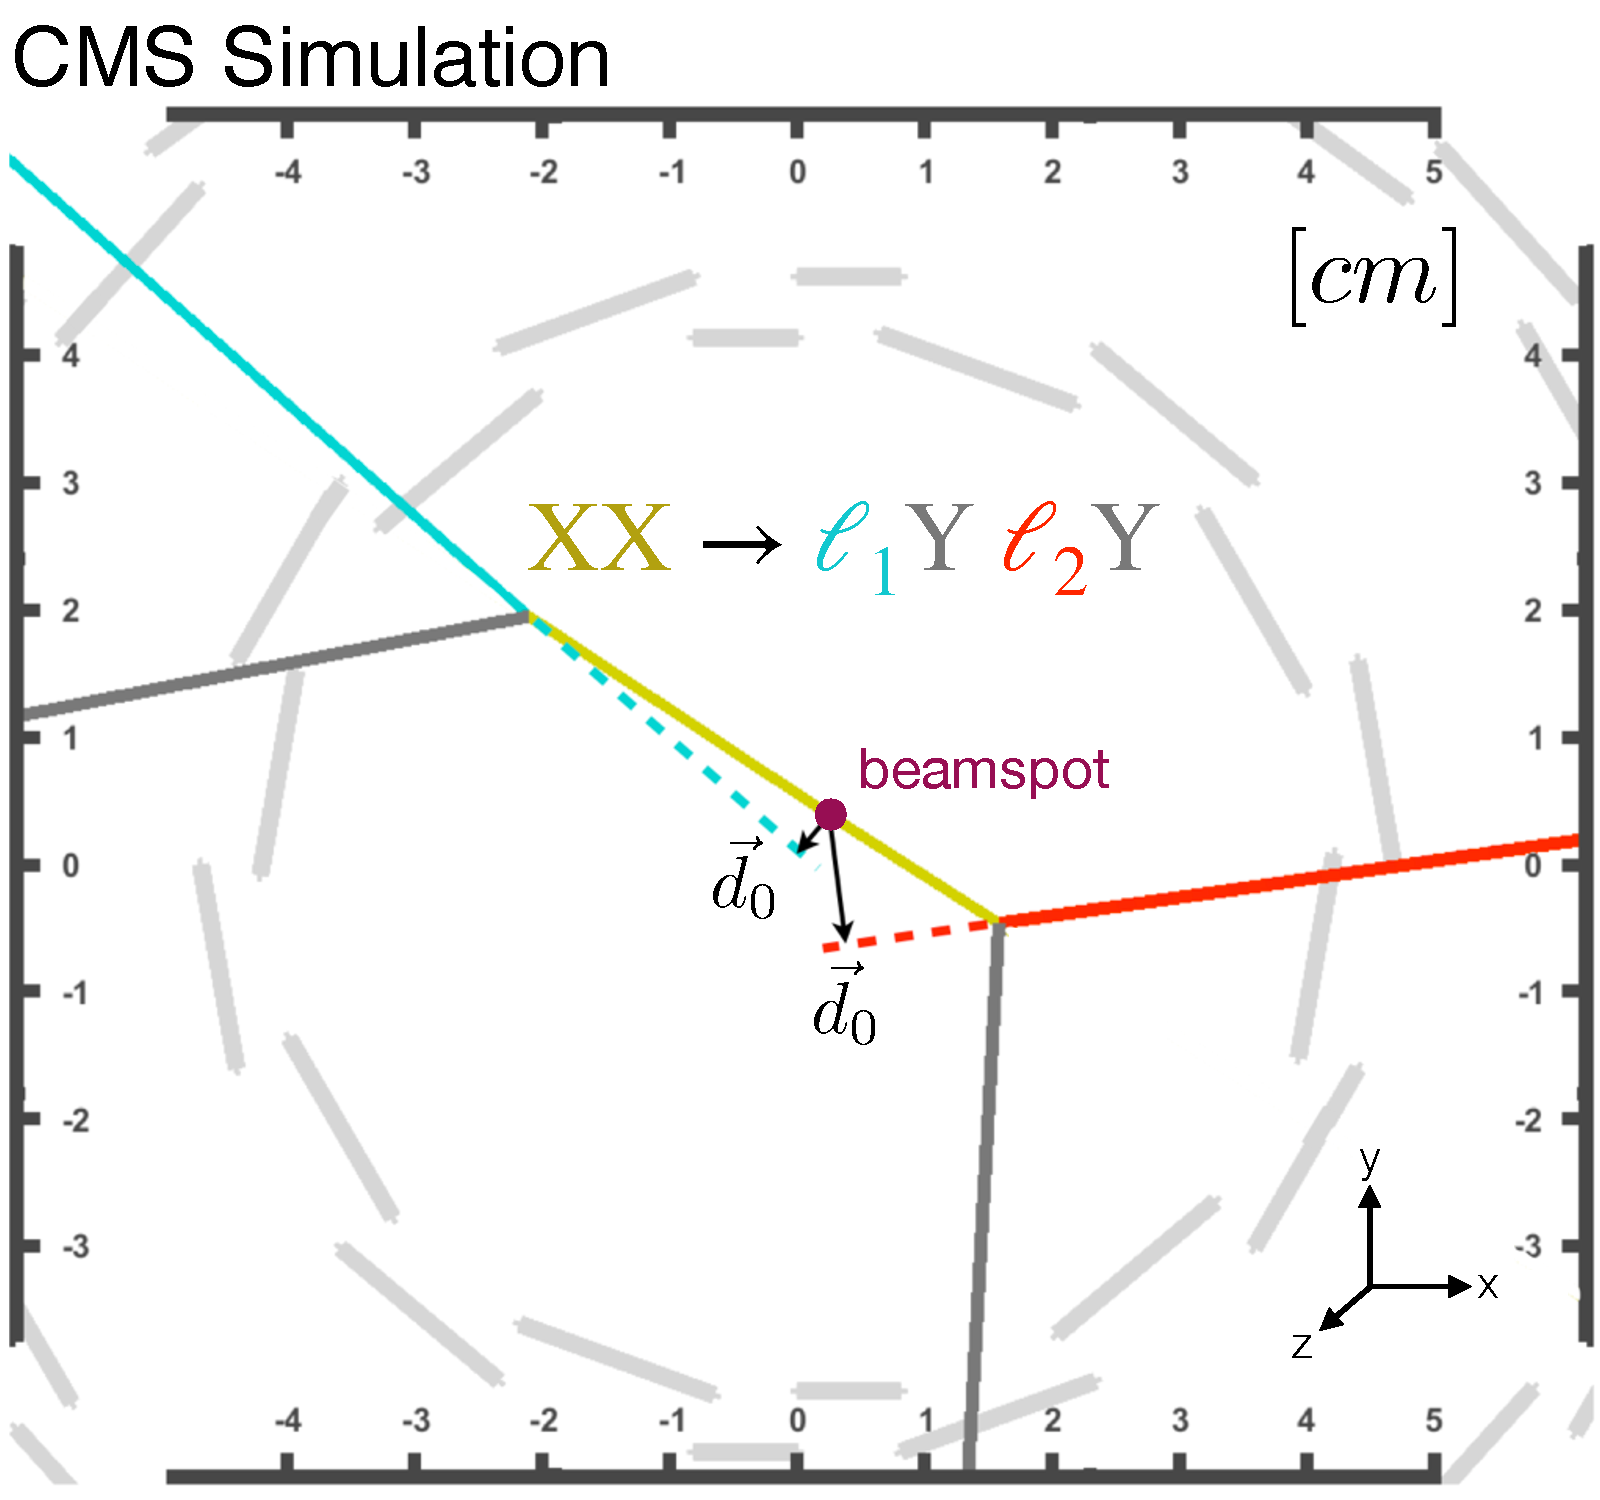
\includegraphics[scale=0.4]{figures/overview/signalEventDisplay.pdf}
\caption{Illustration of the displaced leptons signature showing the definition of $d_0$ in a transverse view of the CMS interaction point. $X$ denotes a new long-lived particle, $\mathcal(l)$ denotes an electron or muon, and $Y$ denotes any other decay products of the new long-lived particle. When interpreting the results of the Displaced Leptons analysis with the Displaced SUSY model, $X$ refers to a top squark and $Y$ refers to a b or d quark.} 
\label{displaced_leptons_cartoon}
\end{figure}